\documentclass[hidelinks]{article}

\usepackage[final,nonatbib]{nips_2016}

\usepackage[pdftex]{graphicx}		% including of figures, etc
\usepackage{float}					% alignment of tables/figures 
\usepackage[utf8]{inputenc} 		% allow utf-8 input
\usepackage[T1]{fontenc}    		% use 8-bit T1 fonts
\usepackage{hyperref}       		% hyperlinks
\usepackage{url}            		% simple URL typesetting
\usepackage{booktabs}       		% professional-quality tables
\usepackage{amsfonts}       		% blackboard math symbols
\usepackage{amsmath}				% math equation stuff
\usepackage[detect-none]{siunitx} 	% si units, range and stuff
\usepackage{nicefrac}       		% compact symbols for 1/2, etc.
\usepackage{microtype}      		% microtypography

% graphicx: Where should graphics be found?
\graphicspath{ {figures/} }

% Setup range symbol.
\sisetup{range-phrase = \text{--}}


% =============================================================================

\title{Deep Features to Track}

\author{Parker Lusk}

\begin{document}

\maketitle

% -----------------------------------------------------------------------------

\begin{abstract}
Almost all vision-based algorithms (deep learning and otherwise) rely on finding a set of lower dimensional features from a higher dimensional image space. In the visual tracking problem, salient features of the target(s) being tracked are selected using one of a variety of feature detector algorithms. Features are then corresponded across video frames and those measurements are passed to a filtering and data association stage. The bottleneck of most target trackers is the vision based frontend. The purpose of this work is to consider the computational efficiency afforded by transfer learning -- using the lower levels of a pretrained network to replace the feature detection part of a visual target tracking system.
\end{abstract}

\section{Introduction}

Almost all vision-based algorithms (deep learning and otherwise) rely on finding a set of lower dimensional features from a higher dimensional image space. In the visual tracking problem, salient features of the target(s) being tracked are selected using one of a variety of feature detector algorithms. Features are then corresponded across video frames and those measurements are passed to a filtering and data association stage. The bottleneck of most target trackers is the vision based frontend. The purpose of this work is to consider the computational efficiency afforded by transfer learning -- using the lower levels of a pretrained network to replace the feature detection part of a visual target tracking system.

% -----------------------------------------------------------------------------

\section{Visual Multiple Target Tracking}
Visual target tracking is an important component of many robotics applications. The need for vision-based tracking in many different settings has given rise to multiple solutions for this problem, each carrying their own assumptions. For example, a popular and well known feature tracker is the Lucas-Kanade Tracker, which uses optical flow to track featuere points across frames. This tracker constrains the camera to be on a static platform and assumes that the track(s) persists in the frame the entire duration of processing. This is a problem for robust tracking solutions

In the BYU MAGICC Lab, visual target tracking is an important subsystem of an integrated unmanned aerial system (UAS), or more colloquially, a drone. Not only is the platform moving, but it is necessary to track multiple dynamic targets that may come into and/or leave the field-of-view of the camera. The Recursive-RANSAC \cite{Niedfeldt2014, Defranco2015} algorithm was developed by the BYU MAGICC Lab to address these concerns.

Recursive-RANSAC is the core algorithm that can handle multiple target tracking in clutter, using a RANSAC approach to initialize tracks and a Kalman filter to update tracks and associate measurements according to a nearly constant acceleration (NCA) motion model. When applied to visual multiple target tracking, R-RANSAC is a powerful tool for generating and predicting the tracks of moving ground targets.

% -----------------------------------------------------------------------------

\section{Feature Detectors}
Many computer vision based algorithms start with the detction and extraction of features from an input image. As a result, many flavours of feature detection have been developed, each with its own strengths and weaknesses. Feature detectors are most robust when the computational complexity is low and there is repeatability of finding the same features given the same input.

There are four common types of image features: \textit{edges}, \textit{corners}, \textit{blobs}, and \textit{ridges}. The Harris and the Shi-Tomasi corner detectors are two methods in wide use today and will be discussed below.

\subsection{Harris Corner Detector}
The Harris corner detector \cite{Harris1988} is an improvement to Moravec's corner detector \cite{Moravec1980}, which considered a window of the image and determined the average changes of image intensity that result from shifting the window by a small amount in prescribed directions. Harris and Stephens mathematically formalized Moravec's heuristic through the eigenvalues of the $2x2$ matrix of the windowed gradients of the image, given by

\begin{equation}
M =
\begin{bmatrix}
  w*I_x^2 & w*I_x I_y \\
  w*I_x I_y & w*I_y^2
\end{bmatrix},
\end{equation}

where $*$ denotes convolution, $w$ is the window (typically Gaussian), and $I_x$ and $I_y$ are the partial derivatives of the image $I$.

By diagonalizing $M$ using eigenvalue decomposition, Harris and Stephens gave meaning to the eigenspace of $M$ as illustrated in \cite[Figure~5]{Harris1988}. Their results show the following for a given pixel $(x_0, y_0)$ in the image $I(x, y)$:

\begin{enumerate}
  \item If $\lambda_1 \approx 0$ and $\lambda_2 \approx 0$ then this region is flat and has no corner.
  \item If $\lambda_1 \approx 0$ and $\lambda_2 \gg 0$ then this region has an edge.
  \item If $\lambda_1 \gg 0$ and $\lambda_2 \gg 0$ then this region has a corner.
\end{enumerate}

Noting that matrix diagonalization can be computationally expensive, Harris and Stephens define a measure of cornered-ness using the properties $tr(M) = \lambda_1 + \lambda_2$ and $det(M) = \lambda_1 \lambda_2$. Their corner/edge response function is defined as

\begin{equation}\label{eq:harris_corn_meas}
  R = det(M) - \kappa\ tr^2(M),
\end{equation}

where $\kappa$ is a tunable sensitivity parameter, empirically found to typically be in the range of \numrange{0.04}{0.15}.

\subsection{Good Features to Track}
Building off of the work of Harris, Stephens, and Moravec, six years after the Harris corner detector paper was published, Shi and Tomasi proposed a different measure of cornered-ness than equation~\ref{eq:harris_corn_meas}:

\begin{equation}
  min(\lambda_1, \lambda_2) > \lambda_{th}.
\end{equation}

If this inequality holds for some threshold $\lambda_{th}$, the current window is accepted. Note that the eigenvalues must be directly computed for this method. The Shi-Tomasi argument is that under certain assumptions, the corners are more stable for tracking.

% -----------------------------------------------------------------------------

\section{Convolutional Neural Networks}

\subsection{Background}
Convolutional Neural Networks (CNNs or ConvNets) are a particular class of deep learning algorithms that have recently proved to be very powerful in image processing tasks. ConvNets are a type of feed-forward deep artificial neural network that consists of layers that process visual information in a hierarchical manner. Each layer is composed of small computational units known as convolutions, which essentially take a weighted average of regions of the input using a small filter (or kernel), typically on the order of a $3x3$ matrix. The weights of these filters are "learned" during back-propagation at test-time. This matrix of weights, or filter, is slide across the entire input to create what is called a feature map: a differently filtered version of the input image. See Figure~\ref{fig:conv_layer} for an illustration of a convolutional layer.

\begin{figure}[H]
  \centering
  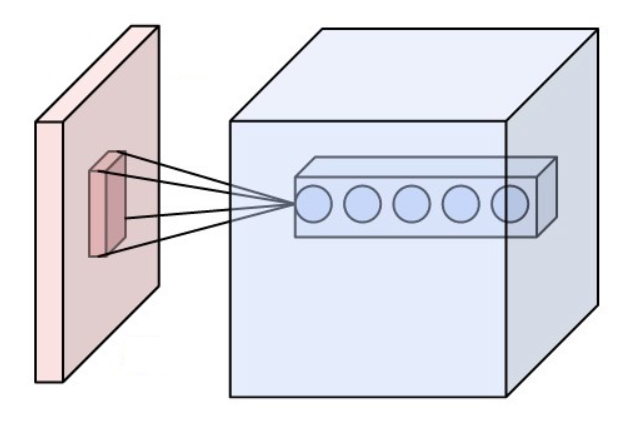
\includegraphics[scale=0.35]{conv_layer}
  \caption{Representation of a convolutional layer, showing an image (left) being scanned by a filter that has different weights at each depth of the output feature maps (right). Any given convolutional layer outputs a set of feature maps, defined by the depth of a layer. See \url{https://en.wikipedia.org/wiki/Convolutional_neural_network}}
  \label{fig:conv_layer}
\end{figure}

These convolutional layers are at the core of CNNs and is why they differ from vanilla deep neural networks (DNNs). A DNN is essentially a multilayer perceptron (MLP) with many hidden fully-connected layers. Because of the inherently spatial nature of images, convolutional layers do better than fully-connected layers as they preserve some level of spatial correlation of features. A typical CNN architecture is shown in Figure~\ref{fig:typical_cnn}.

Convolutional neural networks have been shown to do very well recently in supervised learning, often measured by the ability to classify the natural images from the ImageNet dataset. A flagship example of the power of CNNs is the AlexNet architecture\cite{Krizhevsky2012}, further improved on by the GoogLeNet \cite{Szegedy2014} and VGG \cite{Simonyan2015} architectures. The VGG architecture is shown in Figure~\ref{fig:vgg16}.

\begin{figure}[h]
  \centering
  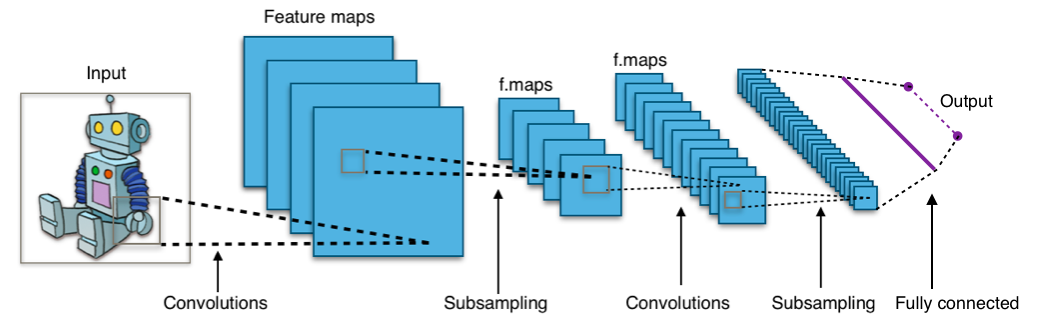
\includegraphics[scale=0.35]{typical_cnn}
  \caption{Typical CNN architecture, consisting mainly of convolutional layers. See \url{https://en.wikipedia.org/wiki/Convolutional_neural_network}}
  \label{fig:typical_cnn}
\end{figure}

\subsection{Visualizing Feature Maps}
With all of the recent advances in deep neural networks in general and with convolutional neural networks in particular, it is becoming increasingly important to understand how they work. Our comprehension of how these models work and what these biologically-inspired neural nets are "thinking" has lagged behind our successes with them. This is especially true in the hidden layers in between the input and output layers.

Work has been progressing in this area, however, as researchers crack open the black box that is ConvNets. A popular method is to generate images that maximize the "activations" (the magnitude of the feature maps) in each layer \cite{Zeiler2014, Yosinski2015, Simonyan2014}. In \cite{Yosinski2015}, Yosinki \textit{et al.} develop a software tool that allows introspection of a convolutional neural network, as shown in Figure~\ref{fig:deepviz}. Use of this tool increases one's intuition of layers and the features that each layer in the hierarchy look for. It turns out that as an image advances in the ConvNet hierarchy, the amount of semantic information increases, i.e., beginning layers pick out task-independent features (edges, corners, etc) while layers toward the end of a CNN pick out more contextual information (book, face, dog, etc).

\begin{figure}[h]
  \centering
  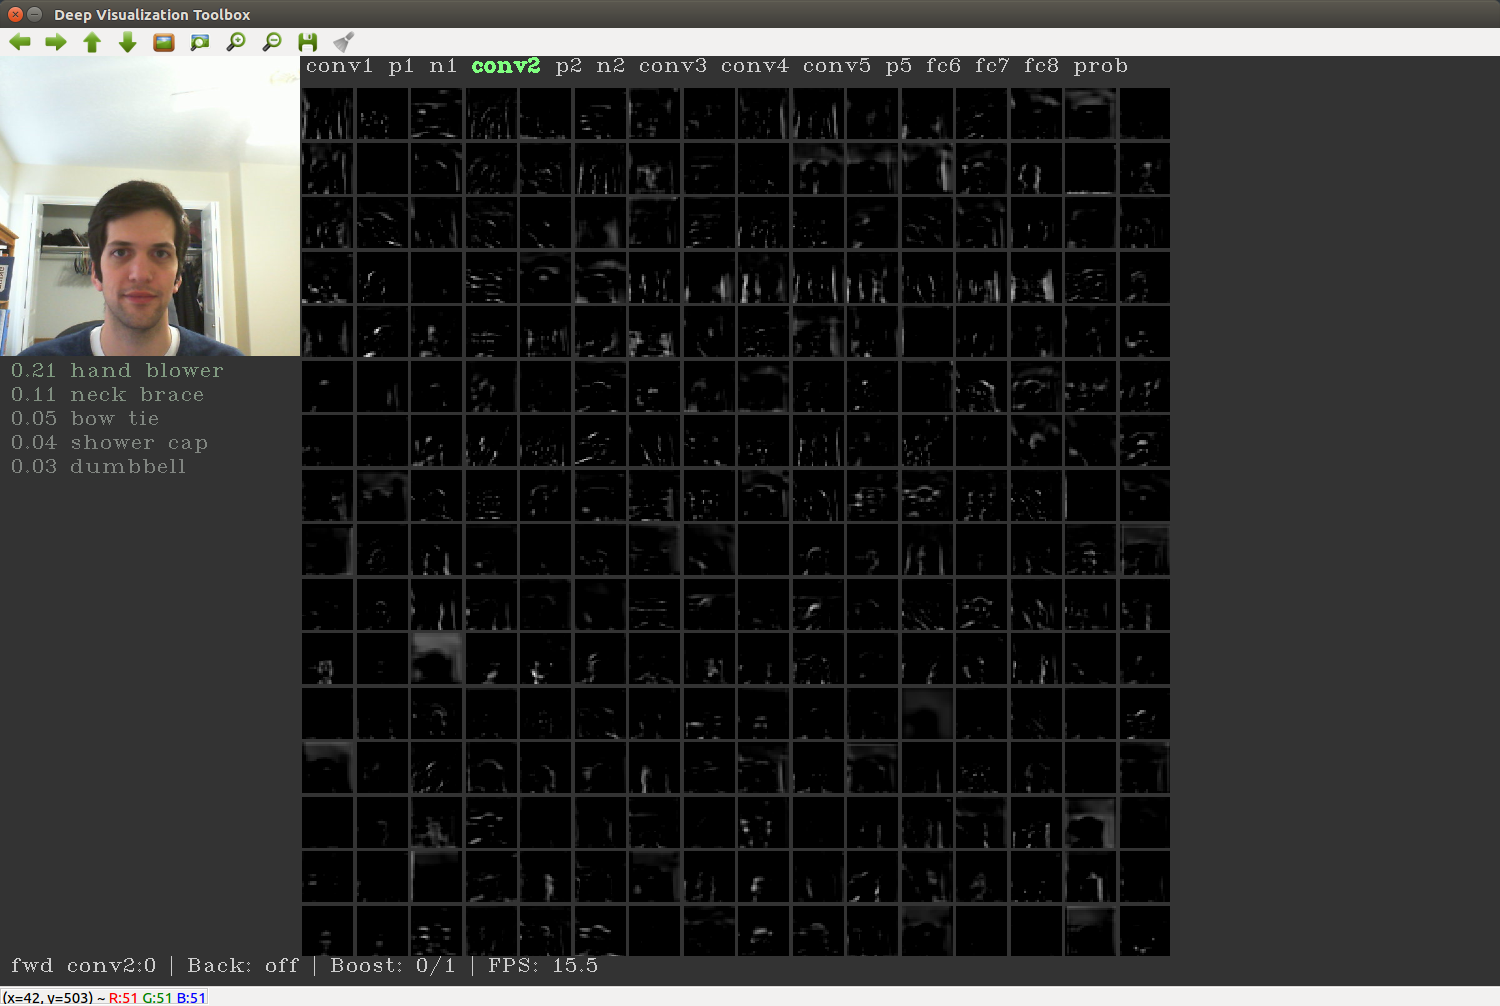
\includegraphics[scale=0.25]{deepviz}
  \caption{Yosinksi's Deep Visualization Toolbox \cite{Yosinski2015}, written in Caffe, running locally and connected to a camera. Note how the feature maps show where the \texttt{conv2} layer has found features from the camera feed of the author.}
  \label{fig:deepviz}
\end{figure}

\subsection{VGG Architecture}

\begin{figure}[H]
  \centering
  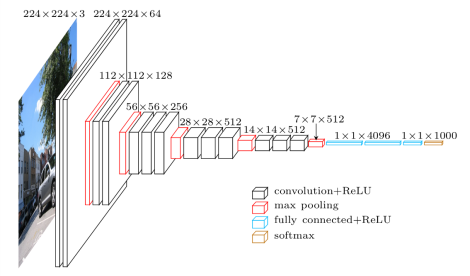
\includegraphics[scale=0.84]{vgg16}
  \caption{Architecture of VGG16 from Oxford's Visual Geometry Group \cite{Simonyan2015}. Taken from \newline \url{https://www.cs.toronto.edu/~frossard/post/vgg16/}.}
  \label{fig:vgg16}
\end{figure}


% -----------------------------------------------------------------------------

\section{Transfer Learning}
Transfer learning refers to the act of training an architecture and then taking a portion of the architecture and weights and using them in another machine learning problem.

% -----------------------------------------------------------------------------

\section{Comparison}

% -----------------------------------------------------------------------------

\section{Conclusion}

\begin{thebibliography}{99}
\small

\bibitem{Niedfeldt2014} P. C. Niedfeldt, “Recursive-RANSAC: A Novel Algorithm for Tracking Multiple Targets in Clutter,” All Theses Diss., no. July, p. Paper 4195, 2014.

\bibitem{Defranco2015} P. C. Defranco, R. W. Beard, K. F. Warnick, and T. W. Mclain, “Detecting and Tracking Moving Objects from a Small Unmanned Air Vehicle,” no. March, 2015.

\bibitem{Shi1994} J. Shi and C. Tomasi, “Good Features to Track,” Pattern Recognit., no. June, 1994.

\bibitem{Harris1988} C. Harris and M. Stephens, “A Combined Corner and Edge Detector,” Procedings Alvey Vis. Conf. 1988, pp. 147–151, 1988.

\bibitem{Moravec1980} H. P. Moravec, “Obstacle avoidance and navigation in the real world by a seeing robot rover.,” tech. Rep. C., p. 175, 1980.

\bibitem{Hong2015} S. Hong, T. You, S. Kwak, and B. Han, “Online Tracking by Learning Discriminative Saliency Map with Convolutional Neural Network,” CoRR, vol. abs/1502.0, 2015.

\bibitem{Krizhevsky2012} A. Krizhevsky, I. Sutskever, and G. E. Hinton, “ImageNet Classification with Deep Convolutional Neural Networks,” Adv. Neural Inf. Process. Syst., pp. 1–9, 2012.

\bibitem{Szegedy2014} C. Szegedy, W. Liu, Y. Jia, P. Sermanet, S. Reed, D. Anguelov, D. Erhan, V. Vanhoucke, A. Rabinovich, C. Hill, and A. Arbor, “Going Deeper with Convolutions,” 2014.

\bibitem{Simonyan2015} K. Simonyan and A. Zisserman, “Very Deep Convolutional Networks for Large-Scale Image Recognition,” Int. Conf. Learn. Represent., pp. 1–14, 2015.

\bibitem{Yosinski2015} J. Yosinski, J. Clune, A. Nguyen, T. Fuchs, and H. Lipson, “Understanding Neural Networks Through Deep Visualization,” Int. Conf. Mach. Learn. - Deep Learn. Work. 2015, p. 12, 2015.

\bibitem{Yosinski2014} J. Yosinski, J. Clune, Y. Bengio, and H. Lipson, “How transferable are features in deep neural networks?,” Adv. Neural Inf. Process. Syst. 27 (Proceedings NIPS), vol. 27, pp. 1–9, 2014.

\bibitem{Zeiler2014} M. D. Zeiler and R. Fergus, “Visualizing and understanding convolutional networks,” Lect. Notes Comput. Sci. (including Subser. Lect. Notes Artif. Intell. Lect. Notes Bioinformatics), vol. 8689 LNCS, no. PART 1, pp. 818–833, 2014.

\bibitem{Simonyan2014} K. Simonyan, A. Vedaldi, and A. Zisserman, “Deep Inside Convolutional Networks: Visualising Image Classification Models and Saliency Maps,” Iclr, p. 1-, 2014.


\end{thebibliography}
\end{document}
